\documentclass[12pt, titlepage]{article}

\usepackage{xcolor} % for different colour comments
\usepackage{tabto}
\usepackage{mdframed}
\mdfsetup{nobreak=true}
\usepackage{xkeyval}
\usepackage{tabularx}
\usepackage{booktabs}
\usepackage{hyperref}
\hypersetup{
    colorlinks,
    citecolor=black,
    filecolor=black,
    linkcolor=red,
    urlcolor=blue
}
\usepackage[skip=2pt, labelfont=bf]{caption}
\usepackage{titlesec}
\usepackage{graphicx}
\graphicspath{ {image/} }



%% the following adds another section level by redefining the paragraph
%% source:  http://tex.stackexchange.com/questions/60209/how-to-add-an-extra-level-of-sections-with-headings-below-subsubsection
\setcounter{secnumdepth}{4}

\titleformat{\paragraph}
{\normalfont\normalsize\bfseries}{\theparagraph}{1em}{}
\titlespacing*{\paragraph}
{0pt}{3.25ex plus 1ex minus .2ex}{1.5ex plus .2ex}


%% Comments
\newif\ifcomments\commentstrue

\ifcomments
\newcommand{\authornote}[3]{\textcolor{#1}{[#3 ---#2]}}
\newcommand{\todo}[1]{\textcolor{red}{[TODO: #1]}}
\else
\newcommand{\authornote}[3]{}
\newcommand{\todo}[1]{}
\fi

\newcommand{\wss}[1]{\authornote{magenta}{SS}{#1}}
\newcommand{\ds}[1]{\authornote{blue}{DS}{#1}}



%% The following are used for pretty printing of events and requirements
\makeatletter

\define@cmdkey      [TP] {test}     {name}       {}
\define@cmdkey      [TP] {test}     {desc}       {}
\define@cmdkey      [TP] {test}     {type}       {}
\define@cmdkey      [TP] {test}     {init}       {}
\define@cmdkey      [TP] {test}     {input}      {}
\define@cmdkey      [TP] {test}     {output}     {}
\define@cmdkey      [TP] {test}     {pass}       {}
\define@cmdkey      [TP] {test}     {user}       {}


\newcommand{\getCurrentSectionNumber}{%
  \ifnum\c@section=0 %
  \thechapter
  \else
  \ifnum\c@subsection=0 %
  \thesection
  \else
  \ifnum\c@subsubsection=0 %
  \thesubsection
  \else
  \thesubsubsection
  \fi
  \fi
  \fi
}

\newcounter{TestNum}

\@addtoreset{TestNum}{section}
\@addtoreset{TestNum}{subsection}
\@addtoreset{TestNum}{subsubsection}

\newcommand{\testauto}[1]{
\setkeys[TP]{test}{#1}
\refstepcounter{TestNum}
\begin{mdframed}[linewidth=1pt]
\begin{tabularx}{\textwidth}{@{}p{3cm}X@{}}
{\bf Test \getCurrentSectionNumber.\theTestNum:} & {\bf \cmdTP@test@name}\\[\baselineskip]
{\bf Description:} & \cmdTP@test@desc\\[0.5\baselineskip]
{\bf Type:} & \cmdTP@test@type\\[0.5\baselineskip]
{\bf Initial State:} & \cmdTP@test@init\\[0.5\baselineskip]
{\bf Input:} & \cmdTP@test@input\\[0.5\baselineskip]
{\bf Output:} & \cmdTP@test@output\\[0.5\baselineskip]
{\bf Pass:} & \cmdTP@test@pass
\end{tabularx}
\end{mdframed}
}

\newcommand{\testmanual}[1]{
\setkeys[TP]{test}{#1}
\refstepcounter{TestNum}
\begin{mdframed}[linewidth=1pt]
\begin{tabularx}{\textwidth}{@{}p{3cm}X@{}}
{\bf Test \getCurrentSectionNumber.\theTestNum:} & {\bf \cmdTP@test@name}\\[\baselineskip]
{\bf Description:} & \cmdTP@test@desc\\[0.5\baselineskip]
{\bf Type:} & \cmdTP@test@type\\[0.5\baselineskip]
{\bf Tester(s):} & \cmdTP@test@user\\[0.5\baselineskip]
{\bf Pass:} & \cmdTP@test@pass
\end{tabularx}
\end{mdframed}
}


\makeatother

\newcommand{\ZtoT}{
\begin{tabularx}{3.85cm}{@{}p{0.35cm}p{0.35cm}p{0.35cm}p{0.35cm}p{0.35cm}p{0.35cm}p{0.35cm}p{0.35cm}p{0.35cm}p{0.35cm}p{0.35cm}@{}}
0 & 1 & 2 & 3 & 4 & 5 & 6 & 7 & 8 & 9 & 10
\end{tabularx}
}

\begin{document}
\title{\bf Physics-Based Chipmunk2D Game\\[\baselineskip]\Large Test Plan}
\author{Steven Palmer\\$\langle$palmes4$\rangle$\\Emaad Fazal\\$\langle$fazale$\rangle$\\Chao Ye\\$\langle$yec6$\rangle$}
\date{\today}
	
\maketitle

\pagenumbering{roman}
\tableofcontents
\listoftables
\listoffigures


\begin{table}[bp]
\caption*{\bf Revision History}
\begin{tabularx}{\textwidth}{p{3.5cm}p{2cm}X}
\toprule {\bf Date} & {\bf Version} & {\bf Notes}\\
\midrule
October 25, 2015 & 1.0 & Created document\\
October 31, 2015 & 1.1 & Major additions to all sections\\
\bottomrule
\end{tabularx}
\end{table}

\newpage

\pagenumbering{arabic}

\section{Overview}
The purpose of this document is to provide a detailed plan for the testing of our game.  The following brief outline gives and overview of what is covered in this document:

\begin{itemize}
  \item A proof of concept test is described in \hyperref[sec:poc]{\S\ref*{sec:poc}}.
  \item System testing is separated into game mechanics testing and game design testing.  The set of tests that will be used in testing the system is described in \hyperref[sec:testing]{\S\ref*{sec:testing}}.
  \item The set of tests that will be used to ensure that the software requirements specifications are met is described in \hyperref[sec:reqtesting]{\S\ref*{sec:reqtesting}}.
  \item A timeline of the test plan is given in \hyperref[sec:timeline]{\S\ref*{sec:timeline}}.  
\end{itemize}

\subsection{Test Case Format}
The description of the tests that will be carried out are formatted in the following way throughout the document: 

\begin{mdframed}[linewidth=1pt]
\begin{tabularx}{\textwidth}{@{}p{3cm}X@{}}
{\bf Test \#:} & {\bf Test name}\\[\baselineskip]
{\bf Description:} & A description of what is being tested\\[0.5\baselineskip]
{\bf Type:} & The type of test\\[0.5\baselineskip]
{\bf Tester(s):} & The people who will run the test ({\bf manual only})\\[0.5\baselineskip]
{\bf Initial State:} & The initial state of the system being tested ({\bf unit test only})\\[0.5\baselineskip]
{\bf Input:} &  The input that will change the state of the system ({\bf unit test only})\\[0.5\baselineskip]
{\bf Output:} & The relevant output that is checked ({\bf unit test only})\\[0.5\baselineskip]
{\bf Pass:} & The pass criteria for the relevant output in the case of unit tests, or a description of the pass criteria for other tests
\end{tabularx}
\end{mdframed}

\subsection{Automated Testing}
Automated testing will be used for testing of the game mechanics system.  Automated tests will include unit testing and coverage analysis.

\subsubsection{Testing Tools}
The software tools that will be used to carry out the automated testing are listed in \hyperref[tab:tools]{Table~\ref*{tab:tools}}

\begin{table}[ht]
\caption{List of testing tools} \label{tab:tools}
\begin{tabularx}{\textwidth}{p{2.3cm}p{4.5cm}X}
\toprule {\bf Tool} & {\bf Description} & {\bf Use}\\
\midrule
gUnit & Unit testing framework & Unit testing\\
COVTOOL & Test coverage analyzer & Analysis of unit test coverage\\
\bottomrule
\end{tabularx}
\end{table}

\subsection{Manual Testing}
Tests that are run manually will be carried out :

\begin{description}
  \item[Game Developers] Blah balh
  \item[Testing Group] A group of $\hyperref[tab:constants]{\delta}$ individuals not involved in the development of the game.  This group will used in two separate testing phases.  Phase I 
\end{description}

The user testing


\subsection{List of Constants}
Constants used in this document are listed in \hyperref[tab:constants]{Table~\ref*{tab:constants}}.
\begin{table}[ht]
\caption{List of constants} \label{tab:constants}
\begin{tabularx}{\textwidth}{p{3cm}p{2cm}X}
\toprule {\bf Constant} & {\bf Value} & {\bf Description}\\
\midrule
$\alpha$ & 5.0 & Hero walk speed\\
$\beta$ & 3.0 & Hero run speed factor: run speed = $\alpha \times \beta$\\
$\gamma$ & 100.0 & Projectile speed\\
$\delta$ & 10 & Number of people in testing group\\
$\epsilon$ & 99\% & Coverage target\\
$\zeta$ & 3.0 & Enemy slow movement speed\\
$\eta$ & 10.0 & Enemy medium movement speed\\
$\theta$ & 30.0 & Enemy fast movement speed\\
\bottomrule
\end{tabularx}
\end{table}

\subsection{Terminology}
Terminology used in this document are listed in \hyperref[tab:terminology]{Table~\ref*{tab:terminology}}.
\begin{table}[ht]
\caption{List of terminology} \label{tab:terminology}
\begin{tabularx}{\textwidth}{p{3cm}X}
\toprule {\bf Term} & {\bf Definition}\\
\midrule
Floor & Horizontal obstacle that hero and enemies cannot pass through\\
Hero & User-controlled character\\
Platform & Horizontal obstacle that hero and enemies cannot pass through from above, but may pass through from below\\
Wall & Vertical obstacle that hero and enemies cannot pass through\\
\bottomrule
\end{tabularx}
\end{table}


\section{Proof of Concept Testing}
\label{sec:poc}
Before any serious development of the game begins, a proof of concept test will be carried out to show that the undertaking is feasible.  The remainder of this section provides detail on what will be used as a proof of concept test.

\subsection{Significant Risks}
The successful completion of the project depends on overcoming the following significant risks:
\begin{enumerate}
  \item In order to use the Chipmunk2D library it must first be successfully compiled.  Since we intend for the game to be compatible with Windows 7, Mac OS X, and Ubuntu, there is a significant risk for the project to fail if compilation is not achieved on all three operating systems.
  \item Chipmunk2D is a large library and its use is not straight forward.  Successful implementation of the library features is crucial to the success of the project and the failure of this poses another significant risk.
\end{enumerate}


\subsection{Demonstration Plan}

For a proof of concept test we will produce a working prototype that can be run on Windows 7, Mac OS X, and Ubuntu.  The prototype will consist of a game demo that implements gravity and collision detection provided by the Chipmunk2D library.  Rudimentary graphics will be used for the prototype since the scope is limited only to demonstrating that the identified risks can be overcome.

The prototype will consist of a small room in which a hero character and enemies exist.  The room will be bounded by a floor below and walls on the left and right, all of which the hero and enemies cannot pass through.  The room will contain platforms which the hero and enemies cannot pass through from above, but may pass through from below when jumping.  A rough idea of the room is given in \hyperref[fig:room]{Figure~\ref*{fig:room}}.

\begin{figure}[ht]
\begin{center}
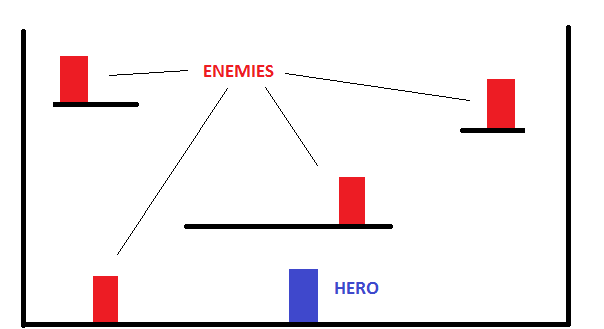
\includegraphics[width=0.75\textwidth]{demo}
\caption{Proof of concept sketch} \label{fig:room}
\end{center}
\end{figure}

The hero character will be represented by a blue rectangle and will be controlled by the user in the following ways:

\begin{itemize}
  \item The hero moves left and right using the 'a' and 'd' keys respectively
  \item The hero jumps by pressing the 'space' key
  \item The hero shoots a projectile in the direction of the mouse cursor by left-clicking
\end{itemize}

Enemies will be represented by red rectangles and will not have any programmed AI (they will not move or attack).  The hero will be able to attack enemies with a projectile, which will knock them back when they are hit.  The hero and all enemies will be subject to gravity and will free-fall when there is no platform or boundary under them.

\subsection{Proof of Concept Test}

\testmanual{
    name = Proof of Concept,
    desc = Tests whether significant risks to the completion of the project can be overcome,
    type = {Proof of Concept (manual)},
    user = Game developers,
    pass = Successful development of a small demonstration which makes use of the Chipmunk2D physics engine
}


\section{System Testing}
\label{sec:testing}
System testing is broken down into game mechanics testing and game design testing phases.  The game mechanics testing phase take place as the game mechanics system is being developed.  Once the game mechanics systems are in place, the .




\subsection{Game Mechanics Testing}
\label{sec:mechanicstesting}
Automated unit testing will be used as the primary method for testing the game mechanics.  The test cases that will be used are outlined in the remainder of this section.
\subsubsection{Input Testing}
The following tests will ensure that user inputs are handled properly.

\testauto{
    name = {Walk left, started from stationary},
    desc = Tests if the hero walks left when the corresponding input is received when the hero is initially stationary,
    type = {Unit Test (dynamic, automated)},
    init = Custom in-game state with hero object having x-velocity of zero,
    input = Keyboard function called with simulated left key down stroke,
    output = Hero object x-velocity (side-effect),
    pass = Hero object x-velocity is $-\hyperref[tab:constants]{\alpha}$
}

\testauto{
    name = {Walk left, started from walking left},
    desc = Tests if the hero walks left when the corresponding input is received when the hero is initially walking left,
    type = {Unit Test (dynamic, automated)},
    init = Custom in-game state with hero object having x-velocity of $-\hyperref[tab:constants]{\alpha}$,
    input = Keyboard function called with simulated left key down stroke,
    output = Hero object x-velocity (side-effect),
    pass = Hero object x-velocity is $-\hyperref[tab:constants]{\alpha}$
}

\testauto{
    name = {Walk left, started from running left},
    desc = Tests if the hero walks left when the corresponding input is received when the hero is initially running left,
    type = {Unit Test (dynamic, automated)},
    init = Custom in-game state with hero object having x-velocity of $-\hyperref[tab:constants]{\beta}\times\hyperref[tab:constants]{\alpha}$,
    input = Keyboard function called with simulated left key down stroke,
    output = Hero object x-velocity (side-effect),
    pass = Hero object x-velocity is $-\hyperref[tab:constants]{\alpha}$
}

\testauto{
    name = {Run left, started from stationary},
    desc = Tests if the hero runs left when the corresponding input is received when the hero is initially stationary,
    type = {Unit Test (dynamic, automated)},
    init = Custom in-game state with hero object having x-velocity of zero,
    input = Keyboard function called with simulated left key down stroke modified by the shift key,
    output = Hero object x-velocity (side-effect),
    pass = Hero object x-velocity is $-\hyperref[tab:constants]{\beta}\times\hyperref[tab:constants]{\alpha}$
}

\testauto{
    name = {Run left, started from walking left},
    desc = Tests if the hero runs left when the corresponding input is received when the hero is initially walking left,
    type = {Unit Test (dynamic, automated)},
    init = Custom in-game state with hero object having x-velocity of $-\hyperref[tab:constants]{\alpha}$,
    input = Keyboard function called with simulated left key down stroke modified by the shift key,
    output = Hero object x-velocity (side-effect),
    pass = Hero object x-velocity is $-\hyperref[tab:constants]{\beta}\times\hyperref[tab:constants]{\alpha}$
}

\testauto{
    name = {Run left, started from running left},
    desc = Tests if the hero runs left when the corresponding input is received when the hero is initially running left,
    type = {Unit Test (dynamic, automated)},
    init = Custom in-game state with hero object having x-velocity of $-\hyperref[tab:constants]{\beta}\times\hyperref[tab:constants]{\alpha}$,
    input = Keyboard function called with simulated left key down stroke modified by the shift key,
    output = Hero object x-velocity (side-effect),
    pass = Hero object x-velocity is $-\hyperref[tab:constants]{\beta}\times\hyperref[tab:constants]{\alpha}$
}

\testauto{
    name = {Walk right, started from stationary},
    desc = Tests if the hero walks right when the corresponding input is received when the hero is initially stationary,
    type = {Unit Test (dynamic, automated)},
    init = Custom in-game state with hero object having x-velocity of zero,
    input = Keyboard function called with simulated right key down stroke,
    output = Hero object x-velocity (side-effect),
    pass = Hero object x-velocity is $\hyperref[tab:constants]{\alpha}$
}

\testauto{
    name = {Walk right, started from walking right},
    desc = Tests if the hero walks right when the corresponding input is received when the hero is initially walking right,
    type = {Unit Test (dynamic, automated)},
    init = Custom in-game state with hero object having x-velocity of $\hyperref[tab:constants]{\alpha}$,
    input = Keyboard function called with simulated right key down stroke,
    output = Hero object x-velocity (side-effect),
    pass = Hero object x-velocity is $\hyperref[tab:constants]{\alpha}$
}

\testauto{
    name = {Walk right, started from running right},
    desc = Tests if the hero walks right when the corresponding input is received when the hero is initially running right,
    type = {Unit Test (dynamic, automated)},
    init = Custom in-game state with hero object having x-velocity of $\hyperref[tab:constants]{\beta}\times\hyperref[tab:constants]{\alpha}$,
    input = Keyboard function called with simulated right key down stroke,
    output = Hero object x-velocity (side-effect),
    pass = Hero object x-velocity is $\hyperref[tab:constants]{\alpha}$
}

\testauto{
    name = {Run right, started from stationary},
    desc = Tests if the hero runs right when the corresponding input is received when the hero is initially stationary,
    type = {Unit Test (dynamic, automated)},
    init = Custom in-game state with hero object having x-velocity of zero,
    input = Keyboard function called with simulated right key down stroke modified by the shift key,
    output = Hero object x-velocity (side-effect),
    pass = Hero object x-velocity is $\hyperref[tab:constants]{\beta}\times\hyperref[tab:constants]{\alpha}$
}

\testauto{
    name = {Run right, started from walking right},
    desc = Tests if the hero runs right when the corresponding input is received when the hero is initially walking right,
    type = {Unit Test (dynamic, automated)},
    init = Custom in-game state with hero object having x-velocity of $\hyperref[tab:constants]{\alpha}$,
    input = Keyboard function called with simulated right key down stroke modified by the shift key,
    output = Hero object x-velocity (side-effect),
    pass = Hero object x-velocity is $\hyperref[tab:constants]{\beta}\times\hyperref[tab:constants]{\alpha}$
}

\testauto{
    name = {Run right, started from running right},
    desc = Tests if the hero runs right when the corresponding input is received when the hero is initially running right,
    type = {Unit Test (dynamic, automated)},
    init = Custom in-game state with hero object having x-velocity of $\hyperref[tab:constants]{\beta}\times\hyperref[tab:constants]{\alpha}$,
    input = Keyboard function called with simulated right key down stroke modified by the shift key,
    output = Hero object x-velocity (side-effect),
    pass = Hero object x-velocity is $\hyperref[tab:constants]{\beta}\times\hyperref[tab:constants]{\alpha}$
}

\testauto{
    name = Stop walking left,
    desc = Tests if hero stops walking left when corresponding input is stopped,
    type = {Unit Test (dynamic, automated)},
    init = Custom in-game state with hero object having x-velocity of $-\hyperref[tab:constants]{\alpha}$,
    input = Keyboard function called with simulated left key up stroke,
    output = Hero object x-velocity (side-effect),
    pass = Hero object x-velocity is zero
}

\testauto{
    name = Stop running left,
    desc = Tests if hero stops running left when corresponding input is stopped,
    type = {Unit Test (dynamic, automated)},
    init = Custom in-game state with hero object having x-velocity of $-\hyperref[tab:constants]{\beta}\times\hyperref[tab:constants]{\alpha}$,
    input = Keyboard function called with simulated left key up stroke,
    output = Hero object x-velocity (side-effect),
    pass = Hero object x-velocity is zero
}

\testauto{
    name = Stop walking right,
    desc = Tests if hero stops walking right when corresponding input is stopped,
    type = {Unit Test (dynamic, automated)},
    init = Custom in-game state with hero object having x-velocity of $\hyperref[tab:constants]{\alpha}$,
    input = Keyboard function called with simulated right key up stroke,
    output = Hero object x-velocity (side-effect),
    pass = Hero object x-velocity is zero
}

\testauto{
    name = Stop running right,
    desc = Tests if hero stops running right when corresponding input is stopped,
    type = {Unit Test (dynamic, automated)},
    init = Custom in-game state with hero object having x-velocity of $\hyperref[tab:constants]{\beta}\times\hyperref[tab:constants]{\alpha}$,
    input = Keyboard function called with simulated right key up stroke,
    output = Hero object x-velocity (side-effect),
    pass = Hero object x-velocity is zero
}

\testauto{
    name = Jump from static object,
    desc = Tests if hero jumps off a static object when corresponding input is received,
    type = {Unit Test (dynamic, automated)},
    init = Custom in-game state with hero object having y-velocity of zero and a bottom edge in contact with a static object,
    input = Keyboard function called with simulated jump key down stroke,
    output = Hero object y-velocity (side-effect),
    pass = Hero object y-velocity is greater than zero
}

\testauto{
    name = Jump from midair not allowed,
    desc = Tests if hero is unable to jump while in midair when corresponding input is received,
    type = {Unit Test (dynamic, automated)},
    init = Custom in-game state with hero object having y-velocity of zero and a bottom edge not in contact with a static object,
    input = Keyboard function called with simulated jump key down stroke,
    output = Hero object y-velocity (side-effect),
    pass = Hero object y-velocity is zero (unchanged)
}

\testauto{
    name = Activate pistol weapon,
    desc = Tests if hero weapon is changes to pistol when corresponding input is received,
    type = {Unit Test (dynamic, automated)},
    init = Custom in-game state with hero object having y-velocity of zero and a bottom edge not in contact with a static object,
    input = Keyboard function called with simulated jump key down stroke,
    output = Hero object y-velocity (side-effect),
    pass = Hero object y-velocity is zero (unchanged)
}

\subsubsection{Static Object Collision Testing}
The following tests will ensure that the collision detection system is working as intended with respect to dynamic objects colliding with static objects.

\testauto{
    name = Wall obstructs hero walking left,
    desc = Tests whether the hero is stopped by a wall object while walking left,
    type = {Unit Test (dynamic, automated)},
    init = Custom in-game state with hero object having x-velocity $-\hyperref[tab:constants]{\alpha}$ situated directly to the right of a wall,
    input = The chipmunk cpSpaceStep function is called, 
    output = Hero object x-velocity (side-effect),
    pass = Hero object x-velocity is 0
}

\testauto{
    name = Wall obstructs hero running left,
    desc = Tests whether the hero is stopped by a wall object while running left,
    type = {Unit Test (dynamic, automated)},
    init = Custom in-game state with hero object having x-velocity $-\hyperref[tab:constants]{\beta}\times\hyperref[tab:constants]{\alpha}$ situated directly to the right of a wall,
    input = The chipmunk cpSpaceStep function is called,
    output = Hero object x-velocity (side-effect),
    pass = Hero object x-velocity is 0
}

\testauto{
    name = Wall obstructs hero walking right,
    desc = Tests whether the hero is stopped by a wall object while walking right,
    type = {Unit Test (dynamic, automated)},
    init = Custom in-game state with hero object having x-velocity $\hyperref[tab:constants]{\alpha}$ situated directly to the left of a wall,
    input = The chipmunk cpSpaceStep function is called,
    output = Hero object x-velocity (side-effect),
    pass = Hero object x-velocity is 0
}

\testauto{
    name = Wall obstructs hero running right,
    desc = Tests whether the hero is stopped by a wall object while running right,
    type = {Unit Test (dynamic, automated)},
    init = Custom in-game state with hero object having x-velocity $\hyperref[tab:constants]{\beta}\times\hyperref[tab:constants]{\alpha}$ situated directly to the left of a wall,
    input = The chipmunk cpSpaceStep function is called,
    output = Hero object x-velocity (side-effect),
    pass = Hero object x-velocity is 0
}

\testauto{
    name = Floor supports hero from below,
    desc = Tests whether the hero is supported by a floor object,
    type = {Unit Test (dynamic, automated)},
    init = Custom in-game state with hero object having x-velocity $\hyperref[tab:constants]{\beta}\times\hyperref[tab:constants]{\alpha}$ situated directly to the left of a wall,
    input = The chipmunk cpSpaceStep function is called,
    output = Hero object x-velocity (side-effect),
    pass = Hero object x-velocity is 0
}

\testauto{
    name = Floor supports hero from below,
    desc = Tests whether the hero is supported by a floor object,
    type = {Unit Test (dynamic, automated)},
    init = Custom in-game state with hero object having x-velocity $\hyperref[tab:constants]{\beta}\times\hyperref[tab:constants]{\alpha}$ situated directly to the left of a wall,
    input = The chipmunk cpSpaceStep function is called,
    output = Hero object x-velocity (side-effect),
    pass = Hero object x-velocity is 0
}

\testauto{
    name = {Wall obstructs enemy moving left, low speed},
    desc = Tests whether an enemy is stopped by a wall object while walking left,
    type = {Unit Test (dynamic, automated)},
    init = Custom in-game state with hero object having x-velocity $-\hyperref[tab:constants]{\alpha}$ situated directly to the right of a wall,
    input = The chipmunk cpSpaceStep function is called,
    output = Hero object x-velocity (side-effect),
    pass = Hero object x-velocity is 0
}

\testauto{
    name = {Wall obstructs enemy moving left, medium speed},
    desc = Tests whether an enemy is stopped by a wall object while walking left,
    type = {Unit Test (dynamic, automated)},
    init = Custom in-game state with hero object having x-velocity $-\hyperref[tab:constants]{\alpha}$ situated directly to the right of a wall,
    input = The chipmunk cpSpaceStep function is called,
    output = Hero object x-velocity (side-effect),
    pass = Hero object x-velocity is 0
}

\testauto{
    name = {Wall obstructs enemy moving left, high speed},
    desc = Tests whether an enemy is stopped by a wall object while walking left,
    type = {Unit Test (dynamic, automated)},
    init = Custom in-game state with hero object having x-velocity $-\hyperref[tab:constants]{\alpha}$ situated directly to the right of a wall,
    input = The chipmunk cpSpaceStep function is called,
    output = Hero object x-velocity (side-effect),
    pass = Hero object x-velocity is 0
}

\testauto{
    name = {Wall obstructs enemy moving right, low speed},
    desc = Tests whether an enemy is stopped by a wall object while running left,
    type = {Unit Test (dynamic, automated)},
    init = Custom in-game state with enemy object having x-velocity $\hyperref[tab:constants]{\zeta}$ situated directly to the left of a wall object,
    input = The chipmunk cpSpaceStep function is called,
    output = Hero object x-velocity (side-effect),
    pass = Hero object x-velocity is 0
}

\testauto{
    name = {Wall obstructs enemy moving right, medium speed},
    desc = Tests whether an enemy is stopped by a wall object while walking right,
    type = {Unit Test (dynamic, automated)},
    init = Custom in-game state with hero object having x-velocity $\hyperref[tab:constants]{\eta}$ situated directly to the left of a wall object,
    input = The chipmunk cpSpaceStep function is called,
    output = Hero object x-velocity (side-effect),
    pass = Hero object x-velocity is 0
}

\testauto{
    name = {Wall obstructs enemy moving right, high speed},
    desc = Tests whether an enemy is stopped by a wall object while moving right at high speed,
    type = {Unit Test (dynamic, automated)},
    init = Custom in-game state with hero object having x-velocity $\hyperref[tab:constants]{\theta}$ situated directly to the left of a wall object,
    input = The chipmunk cpSpaceStep function is called,
    output = Hero object x-velocity (side-effect),
    pass = Hero object x-velocity is 0
}


\subsubsection{Dynamic Object Collision Testing}
The following tests will ensure that the collisions between dynamic objects work as intended.

\testauto{
    name = Hero projectile collides with enemy,
    desc = Tests whether a projectile launched by the hero collides with enemies,
    type = {Unit Test (dynamic, automated)},
    init = Custom in-game state with a hero projectile object with an x-velocity $-\hyperref[tab:constants]{\gamma}$ located directly to the right of an enemy object,
    input = The chipmunk cpSpaceStep function is called,
    output = State of the space,
    pass = Hero projectile object is removed from the space
}

\testauto{
    name = Enemy projectile collides with hero,
    desc = Tests whether a projectile launched by an enemy collides with the hero,
    type = {Unit Test (dynamic, automated)},
    init = Custom in-game state with an enemy projectile object with an x-velocity $-\hyperref[tab:constants]{\gamma}$ located directly to the right of the hero object,
    input = The chipmunk cpSpaceStep function is called,
    output = State of the space,
    pass = Enemy projectile object is removed from the space
}

\subsubsection{Artificial Intelligence Testing}

\subsubsection{Save/Load Testing}
The following tests will ensure that the game's saving and loading functions work properly.

\testauto{
    name = Load file from menu,
    desc = Tests whether a saved game can be successfully loaded from the main menu,
    type = {Unit Test (dynamic, automated)},
    init = Main menu state,
    input = Load game function is called with file name,
    output = Game state,
    pass = Game state is equal to a predefined state that corresponds exactly to the file
}

\testauto{
    name = {Load file from menu, file does not exist},
    desc = Tests that exception is thrown if a non-existent file is attempted to be loaded,
    type = {Unit Test (dynamic, automated)},
    init = Main menu state,
    input = Load game function is called with a non-existent file name,
    output = File does not exist exception,
    pass = File does not exist exception is thrown and handled
}

\testauto{
    name = Load file from menu,
    desc = Tests whether a saved game can be successfully loaded from the main menu,
    type = {Unit Test (dynamic, automated)},
    init = Main menu state,
    input = Load game function is called with file name,
    output = Game state,
    pass = Game state is equal to a predefined state that corresponds exactly to the file
}

\testauto{
    name = Load file from in-game,
    desc = Tests whether a saved game can be successfully loaded while in-game,
    type = {Unit Test (dynamic, automated)},
    init = Custom in-game state different from that described by the saved game file,
    input = Load game function is called with file name,
    output = Game state,
    pass = Game state is equal to a predefined state that corresponds exactly to the file
}



\subsubsection{Unit Test Coverage}
Once the game mechanics and all of the corresponding unit tests have been implemented, .  This will uncover portions of code that were not tested and allow for the design of additional  

\testauto{
    name = Game mechanics coverage,
    desc = Tests that the game mechanics unit testing adequately covers the game mechanics code,
    type = {Structural (dynamic, automated)},
    pass = Coverage of game mechanics code is greater than $\hyperref[tab:constants]{\epsilon}$
}



\subsection{Game Design Testing}
Once the game mechanics systems have been implemented and shown to be working correctly through the testing described in \hyperref[sec:mechanicstesting]{\S\ref*{sec:mechanicstesting}}, the game itself can be built on top.  The design of the game can be broken down into game world design, story/objectives design, graphics, and sound.  Automated testing for this phase would be time-consuming and difficult to implement.  Therefore, all of the game design testing will consist of manual tests.
\subsubsection{Game World Testing}
\testmanual{
    name = All areas reachable,
    desc = Tests that all areas of the game world that are intended to be reachable by the hero are in fact reachable by the hero,
    type = {Functional (dynamic, manual)},
    user = {Development team},
    pass = No areas are unreachable based on thorough .  Alpha testers and beta testers will be asked to note down any
}

\testmanual{
    name = No ``points of no return'',
    desc = Tests that there are no areas of the game world that will cause the hero to become stuck (e.g. inescapable pits),
    type = {Functional (dynamic, manual)},
    user = {Development team},
    pass = Hero does not become stuck on playthrough testing .  Alpha testers and beta testers are asked to note down any
}

\subsubsection{Story/Objectives Testing}



\subsubsection{Graphics Testing}



\subsubsection{Audio Testing}
The following tests will be carried out to ensure that game audio is properly implemented.

\testmanual{
    name = Hero movement sounds,
    desc = Tests if hero movement sounds are properly implemented,
    type = {Functional (dynamic, manual)},
    user = Development team,
    pass = {Appropriate sounds play when hero walks, runs, jumps, etc.} 
}

\testmanual{
    name = Enemy movement sounds,
    desc = Tests if enemy movement sounds are properly implemented,
    type = {Functional (dynamic, manual)},
    user = Development team,
    pass = Appropriate sounds play when enemies move
}

\testmanual{
    name = Weapon fire sound,
    desc = Tests if hero weapon fire sound is properly implemented,
    type = {Functional (dynamic, manual)},
    user = Development team,
    pass = Appropriate sounds play when hero fires weapon
}

\testmanual{
    name = Enemy attack sounds,
    desc = Tests if enemy attack sounds are properly implemented,
    type = {Functional (dynamic, manual)},
    user = Development team,
    pass = Appropriate sounds play when enemies launch attacks
}

\testmanual{
    name = Collision sounds,
    desc = Tests if hero weapon sounds are properly implemented,
    type = {Functional (dynamic, manual)},
    user = Development team,
    pass = Appropriate sounds play when hero fires weapon
}


\subsection{General Testing}
Throughout both of the system testing phases new code will be reviewed after each commit in an attempt to detect any visible errors.

\testmanual{
    name = Code review,
    desc = Code is read through line by line while checking for errors,
    type = {Structural (static, manual)},
    user = Development team,
    pass = No errors found/all errors fixed
}


\section{Requirements Testing}
\label{sec:reqtesting}

Testing will 

\subsection{Functional Requirements Testing}
The functional requirements given in the software requirements specification document should all be implemented in the final version of the game.  Since these requirements contribute to the , explicit testing of the requirements should be  

\testmanual{
    name = Functional requirements are met,
    desc = Game is compared with software requirements specification,
    type = {Functional (dynamic, manual)},
    user = {Development team},
    pass = All functional requirements are met and tested under system testing
}

\subsection{Non-Functional Requirements Testing}
The following tests will be carried out to ensure adherence to the non-functional requirements given in the software requirements specification.

\testmanual{
    name = {User experience, Phase I},
    desc = Game is compared with software requirements specification,
    type = {Structural (static, manual)},
    user = {Testing group},
    pass = 
}

\testmanual{
    name = {User experience, Phase II},
    desc = Game is compared with software requirements specification,
    type = {Structural (static, manual)},
    user = {Testing group},
    pass =
}

\testmanual{
    name = Spelling and grammar check,
    desc = The game uses proper English and is free of any spelling or grammatical errors,
    type = {Functional (dynamic, manual)},
    user = {Development team},
    pass = No spelling or grammatical errors are detected or all detected errors are corrected
}



\section{Timeline}
\label{sec:timeline}
The testing 




\newpage
\section{Appendix A:  Testing Survey}
\label{sec:survey}

The following survey will be filled out by members of the alpha and beta testing groups.

\begin{mdframed}[linewidth=1pt]
\begin{center}
{\bf \large User Experience Survey}\\[\baselineskip]
\end{center}

\noindent The following survey should be filled out after playing the game for at least 30 minutes.\\

\noindent {\bf Time played:}\\

\noindent Please provide a ranking between 0 and 10 in each of the following categories.  Please include notes on what you did and did not like, and what could be done to improve the game.\\[\baselineskip]

\noindent \begin{tabularx}{\textwidth}{@{}p{3.5cm}X@{}}
{\bf Entertainment:} & \ZtoT \\
& {[~0 = most boring, 10 = most fun~]}\\[\baselineskip]
{\bf Difficulty:} & \ZtoT\\
& {[~0 = easiest, 10 = most difficult~]}\\[\baselineskip]
{\bf Controls:} & \ZtoT\\
& {[~0 = non-intuitive, 10 = intuitive~]}\\[\baselineskip]
{\bf Notes:} & \\[5\baselineskip]
\end{tabularx}
\end{mdframed}



\end{document}
